\chapter{System Development}
\label{chap:Chapter4}

This chapter addresses the most relevant technologies to be considered in this Thesis, according to its objectives.
It highlights different battery technologies, types of external memories and storage units, computing systems, firmware strategies and wireless communication technologies.
%-------------------------------------------------------------------------------%

\section{Battery Module}

Batteries are a critical component in portable embedded systems, providing the necessary energy for the system to work properly.

This way, the battery technology selection must be carefully made to optimize the system performance, \cite{BATT3}.
Different battery chemistries offer varying energy densities, voltages, sizes, weights, cycle lives and costs.

%\subsection{Lithium}
\gls{Li-ion} and \gls{Li-Po} batteries, shown in figures \ref{fig:18650} and \ref{fig:lipo}, can offer high energy density, rechargeability and moderate costs that make them suitable for portable devices, \cite{BATT7}.

These batteries stand out as a prevalent choice for embedded systems.
\begin{figure}[H]
    \centering
    \begin{minipage}{.5\textwidth}
        \centering
        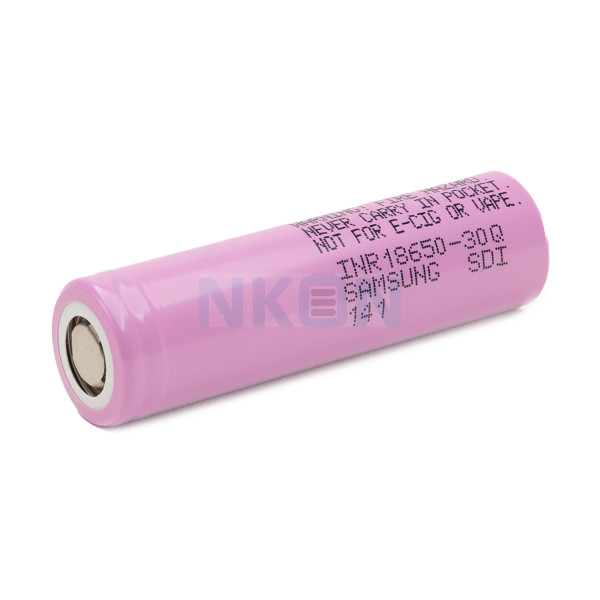
\includegraphics[width=.5\linewidth]{ch4/assets/18650.jpg}
        \captionof{figure}{\gls{Li-ion} battery example \cite{18650}}
        \label{fig:18650}
    \end{minipage}%
    \begin{minipage}{.5\textwidth}
        \centering
        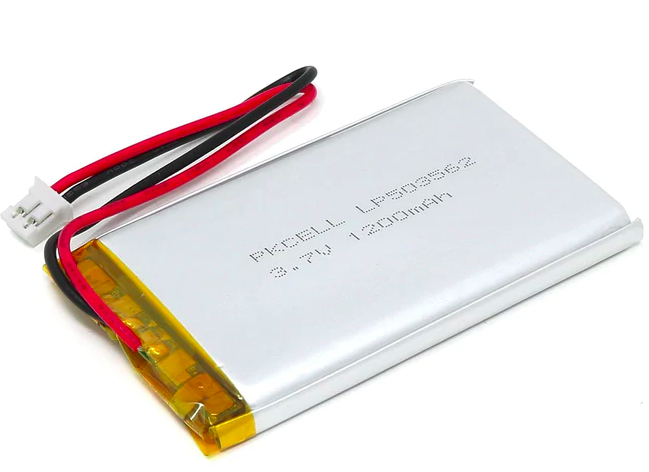
\includegraphics[width=.5\linewidth]{ch4/assets/lipo.png}
        \captionof{figure}{\gls{Li-Po} battery example \cite{lipo}}
        \label{fig:lipo}
    \end{minipage}
\end{figure}

%\subsection{Nickel}
\gls{NiMH} and \gls{NiCd} batteries (figures \ref{fig:NiMH} and \ref{fig:NiCd} respectably) can provide moderate energy density, rechargeability and moderate costs, but they can be heavier and \gls{NiCd} batteries have a \textit{memory effect} concern (where the battery, falsely, indicates full charge despite being only partially charged).
\begin{figure}[H]
    \centering
    \begin{minipage}{.5\textwidth}
        \centering
        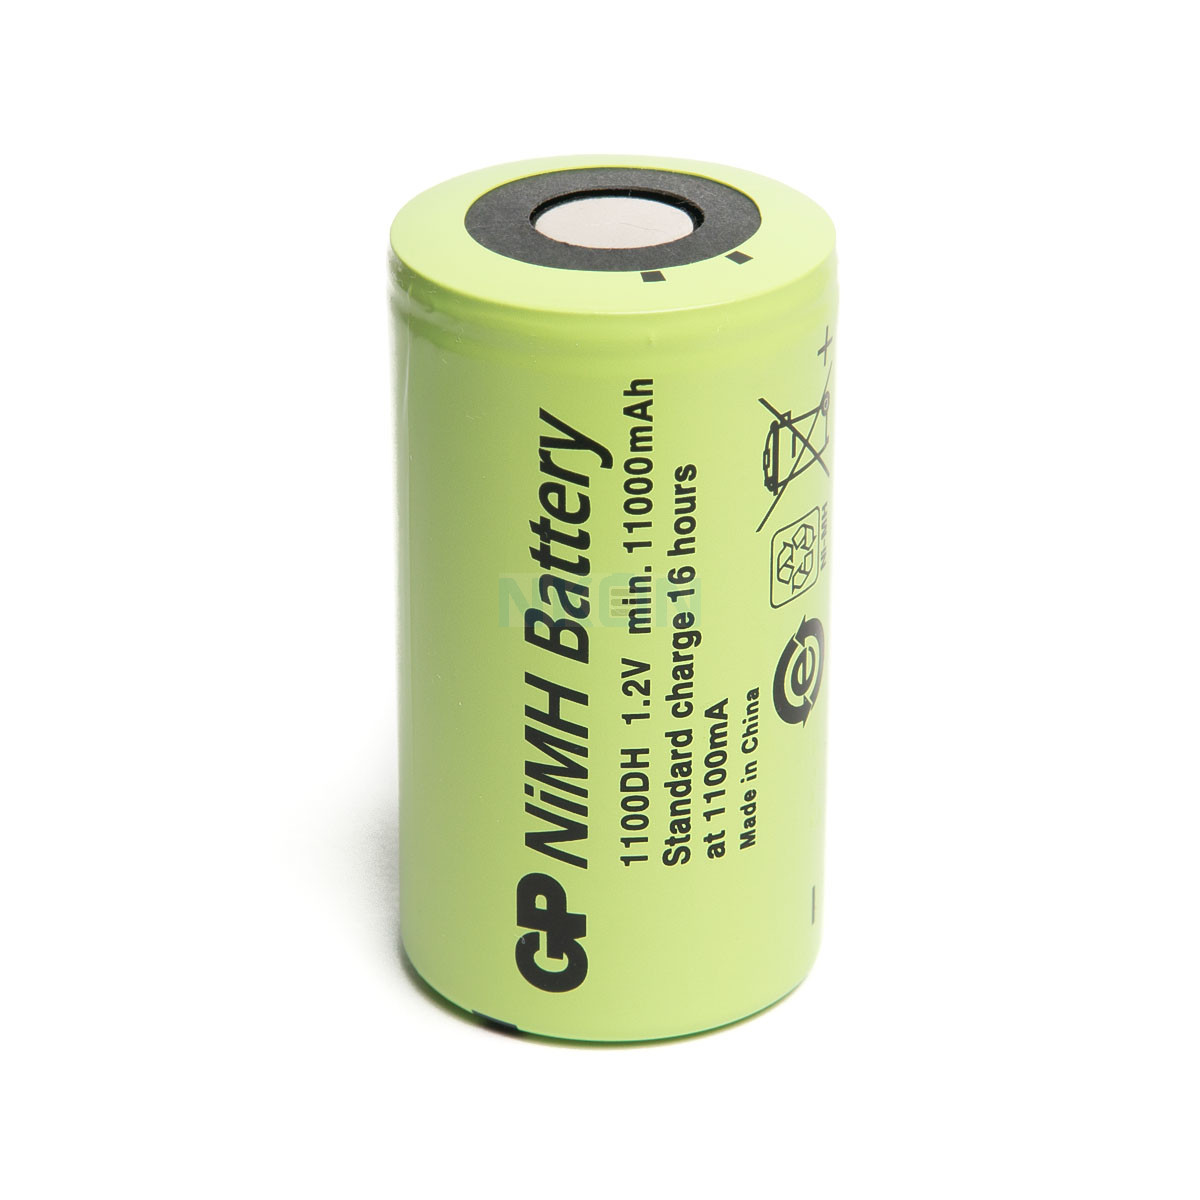
\includegraphics[width=.5\linewidth]{ch4/assets/nimh.jpg}
        \captionof{figure}{\gls{NiMH} battery example \cite{nimh}}
        \label{fig:NiMH}
    \end{minipage}%
    \begin{minipage}{.5\textwidth}
        \centering
        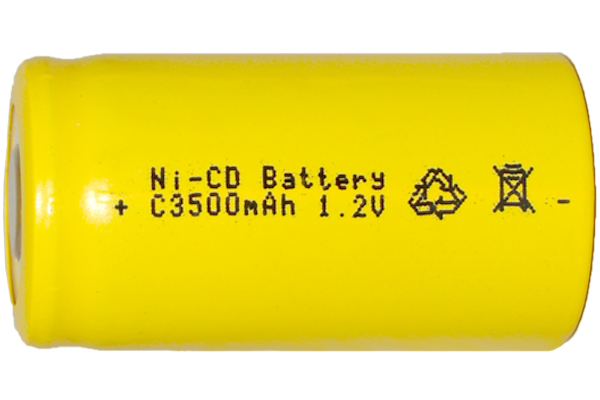
\includegraphics[width=.5\linewidth]{ch4/assets/nicd.jpg}
        \captionof{figure}{\gls{NiCd} battery example \cite{nicd}}
        \label{fig:NiCd}
    \end{minipage}
\end{figure}

%\subsection{Lead-acid}

Lead-acid batteries can be rechargeable and cost-effective but heavier and larger and with low energy density.
These batteries are suitable for less portable applications, \cite{BATT3} as it is possible to see in figure \ref{fig:lead}.
\begin{figure}[H]
    \centering
    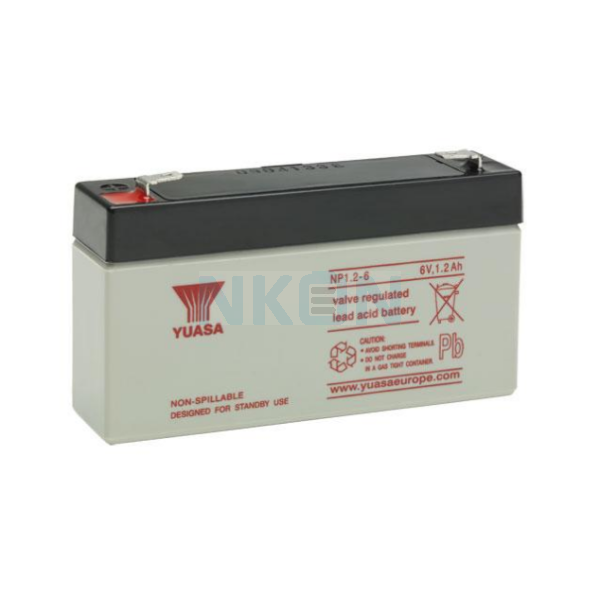
\includegraphics[scale=0.4]{ch4/assets/lead.png}
    \caption{Lead-Acid battery example \cite{lead}}
    \label{fig:lead}
\end{figure}

%\subsection{Alkaline}
Alkaline batteries, in figure \ref{fig:alkaline}, are cost-effective but most of them are non-rechargeable, have a standard cylindrical format and have moderate energy density \cite{BATT3}.
\begin{figure}[H]
    \centering
    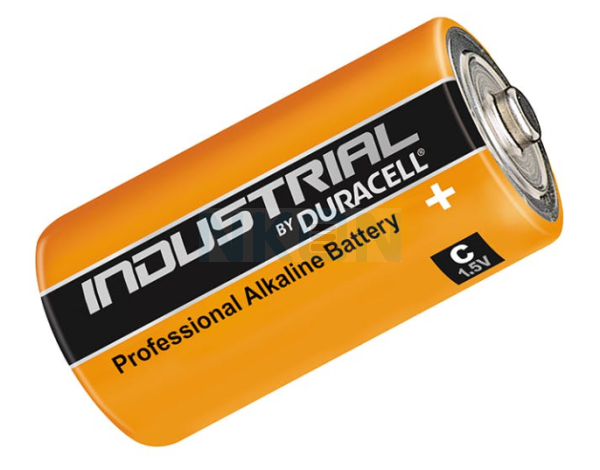
\includegraphics[scale=0.3]{ch4/assets/alkaline.png}
    \caption{Alkaline battery example \cite{alkaline}}
    \label{fig:alkaline}
\end{figure}

\subsection{Battery Technologies Comparison}
In table \ref{tab:battery_comparison} it is possible to see the resume and comparison between the battery technologies examples described previously.
\begin{table}[H]
    \centering
    \resizebox{\textwidth}{!}{
        \begin{tabular}{lccccc}
            \hline
            \textbf{Technology} & \begin{tabular}[c]{@{}c@{}}\textbf{Energy}\\ \textbf{Density}\end{tabular} & \textbf{Voltage} & \textbf{Size/Weight} & \textbf{Cycle Life} & \textbf{Cost} \\ \hline
            \textbf{Li-ion}     & High                                                                       & 3.7V             & Compact/Light        & Good                & Moderate      \\
            \textbf{Li-Po}      & High                                                                       & 3.7V             & Flexible/Light       & Good                & Moderate      \\
            \textbf{NiMH}       & Moderate                                                                   & 1.2V             & Bulky/Heavy          & Moderate            & Moderate      \\
            \textbf{NiCd}       & Moderate                                                                   & 1.2V             & Bulky/Heavy          & Good                & Moderate      \\
            \textbf{Lead-Acid}  & Low                                                                        & 2V (6V, 12V)     & Bulky/Heavy          & Moderate            & Low           \\
            \textbf{Alkaline}   & Moderate                                                                   & 1.5V             & Standard Cylindrical & Poor                & Moderate      \\
        \end{tabular}%
    }
    \caption{Comparison of Battery Technologies}
    \label{tab:battery_comparison}
\end{table}

In this Thesis, the energy density of the battery will be a key characteristic when choosing a battery module.
To avoid adding too much weight to the \gls{uav} and to be able to integrate this solution easily the battery should be small but with high capacity.
%-------------------------------------------------------------------------------%

\section{External Memory and Storage Units}

Memory units can be classified as volatile memory and as non-volatile memory \cite{mem3}.

Volatile storage, like for example \gls{RAM} provides fast read and write speeds and is used for storing variables and managing application stacks.
However, they require constant power to retain data, making them unsuitable for applications with strict power constraints and have lower memory capacity \cite{mem8}.

Non-volatile storages are suitable for applications requiring frequent data read and write operations and have the capability of being electrically erased and reprogrammed.
They have long-term data retention and low power consumption but have slow access speed compared to volatile storage \cite{mem8}.
These characteristics make non-volatile storages useful for storing configuration parameters and critical data that need to be retained during power cycles.

Often, in embedded systems, the system must be able to store data not only internally (main memory) but also externally (external memory).
External memory units are normally used to expand storage capacity, store data and logs, facilitate data transfer, and backup critical information \cite{mem3}.

Since non-volatile storage can keep the data stored even when they are not powered, these storages are very common in embedded systems \cite{mem1}.

%\subsection{\gls{SD} card}
\gls{SD} card, with its multiple formats and sizes, has moderate access speed and can keep data for a long term but it depends on the type (\gls{SLC}, \gls{MLC} and \gls{TLC}).
Typically, the capacity ranges from a few megabytes to multiple terabytes, offering multiple choices for different use cases \cite{mem11}, \cite{mem9}.
However, the moderate power consumption and overall cost can, sometimes, be a setback to the system.

%\subsection{\gls{EEPROM}}
\gls{EEPROM}, commonly used for storing small amounts of data, has fast access speed and a moderate overall cost.
Has long-term data retention and low power consumption but offers lower capacities (in the range of kilobytes to megabytes) making it only suitable for small data storage \cite{mem8}, \cite{mem11}.

%\subsection{\gls{FRAM}}
\gls{FRAM} combines the benefits of \gls{RAM} and \gls{EEPROM} and can be suitable for applications requiring fast and non-volatile memory.
Has very fast access speed, long-term data retention, low capacity (in the range of kilobytes to megabytes), and very low power consumption.
But has a relatively higher overall cost compared to other technologies \cite{mem8}, \cite{mem11}.

%\subsection{\gls{eMMC}}
As for \gls{eMMC}, normally found in smartphones, tablets, and other embedded systems, is characterized by its fast access speed, long-term data retention and high capacity (with ranges from megabytes to terabytes).
Like \gls{SD} cards it has moderate power consumption and moderate to high overall cost \cite{mem11}.

%\subsection{Drives}
\gls{HDD} and \gls{SSD} memory units can have fast access speed, long-term data retention and high capacity (in the range of gigabytes to terabytes).
But, in comparison to other memory units, it has a bigger size, higher power consumption and higher overall cost.
These units are normally used as primary storage in computers and laptops for improved performance, \cite{mem10}.

\subsection{External Memory Technologies Comparison}
Table \ref{tab:memory_comparison} resumes and compares the described technologies in their access speed, overall cost, data retention, capacity and power consumption.
\begin{table}[H]
    \centering
    \resizebox{\textwidth}{!}{
        \begin{tabular}{lccccccc}
            \hline
                              & \textbf{Access Speed} & \textbf{Overall Cost} & \textbf{Data Retention} & \textbf{Capacity} & \textbf{Power Consumption} & \textbf{Ease of Access} \\ \hline
            \textbf{SD Cards} & Moderate              & Moderate              & Long-term               & High              & Moderate                   & Easy                    \\
            \textbf{EEPROM}   & Fast                  & Moderate              & Long-term               & Low               & Low                        & Difficult               \\
            \textbf{FRAM}     & Very Fast             & Relatively Higher     & Long-term               & Low               & Very Low                   & Difficult               \\
            \textbf{eMMC}     & Fast                  & Moderate              & Long-term               & High              & Moderate                   & Easy                    \\
            \textbf{SSD}      & Very Fast             & High                  & Long-term               & Very High         & High                       & Easy                    \\
            \textbf{HDD}      & Moderate              & High                  & Long-term               & Very High         & High                       & Easy                    \\\hline
        \end{tabular}
    }\caption{Comparison of External Memory Technologies}
    \label{tab:memory_comparison}
\end{table}

The external memory, or storage unit, will play an important role in this system.
The ability to store system logs and other types of data will not only help to debug during tests but it will also help to evaluate the system performance.

Thus for this Thesis, the external memory should be able to retain data for long periods, have a high capacity, have a moderate to low power consumption and have easy access to the stored data.

%-------------------------------------------------------------------------------%

\section{Computing Systems and Firmware}

\subsection{Computing Systems}
An \gls{OBC} is a device capable of managing and/or controlling various functions such as:
\begin{itemize}
    \item Manage overall system operation.
    \item Implement safety mechanisms and respond to abnormal conditions.
    \item Execute algorithms and computations required for the system's functionality.
    \item Interface with external devices, sensors, actuators, or other embedded systems.
    \item Implement communication protocols for data exchange.
    \item Manage data storage and retrieval.
    \item Implement power-saving modes when appropriate.
    \item Manage and control peripherals such as communication interfaces, timers, and interrupt controllers.
\end{itemize}

There are, mainly, three types of control units: \textbf{Microcontrollers}, \textbf{Microprocessors}, and \textbf{\glspl{FPGA}}.

\textbf{Microcontrollers} are integrated circuits that, mainly, contain a processor core, memory, and programmable input/output peripherals.
Since they are compact and have low power consumption, they can be designed for specific tasks which makes them suitable for embedded systems.
They often include integrated peripherals like timers, communication interfaces (for example \gls{I2C}, \gls{SPI}, \gls{CAN} and \gls{UART}), \gls{ADC} and \gls{RTC} \cite{OBC1}.

Microcontrollers are programmable using low-level programming languages like C, C++ and Assembly \cite{OBC1}.

However, microcontrollers have more limited processing power and are less flexible for general-purpose computing \cite{OBC1} and \cite{OBC2}.

\textbf{Microprocessors} focus on processing tasks and rely on external components for additional functionalities.
As an advantage, they have high processing power (suitable for general-purpose computing), can run complex operating systems, and have greater flexibility in application design.
They can also be programmed by low-level or high-level programming languages which facilitates the development of firmware \cite{OBC5}.

However, microprocessors have higher power consumption, may require additional components for specific applications, and have a larger form factor compared to microcontrollers \cite{OBC5}.

\textbf{\glspl{FPGA}} are integrated circuits that can be configured after manufacturing, allowing for custom circuits.
The \gls{FPGA} architecture is composed of configurable logic blocks that a developer can program making them highly customizable for specific applications.
It has parallel processing capabilities and can be reprogrammed for different tasks \cite{OBC1}, \cite{OBC3} and \cite{OBC5}.

But, they have a higher cost and higher power consumption (compared to microcontrollers).
Since programming \gls{FPGA} is done by programming the hardware (with \gls{HDL}), the method is different from programming a microcontroller (with specific software) the learning curve can be steeper \cite{OBC1} \cite{OBC3}.

\subsubsection{Computing System Technologies Comparison}
The table \ref{tab:obc_comparison} compares the programming languages, flexibility, processing power, development complexity, cost, real-time performance and power consumption of these three main types of control units \cite{OBC5}.
\begin{table}[H]
    \centering
    \resizebox{\textwidth}{!}{
        \begin{tabular}{lccc}
            \hline
            \textbf{Topic}                  & \textbf{Microcontrollers} & \textbf{Microprocessors} & \textbf{FPGAs} \\ \hline
            \textbf{Programming Languages}  & Low-level languages       & High-level languages     & HDL            \\
            \textbf{Flexibility}            & Low                       & Moderate                 & High           \\
            \textbf{Processing Power}       & Limited                   & High                     & High           \\
            \textbf{Development Complexity} & Low                       & Moderate                 & High           \\
            \textbf{Cost Considerations}    & Low                       & Moderate                 & High           \\
            \textbf{Real-time Performance}  & Moderate                  & Low                      & High           \\
            \textbf{Power Consumption}      & Low                       & Moderate to high         & Moderate       \\ \hline
        \end{tabular}
    }
    \caption{Comparison of Microcontrollers, Microprocessors, and FPGAs.}
    \label{tab:obc_comparison}
\end{table}

When choosing the \gls{OBC} for this Thesis, the first characteristic to be analyzed should be the availability to be programmed easily (being by a low-level language, an high-level language or a \gls{RTOS}).
This selection will dictate the firmware strategy.

Other characteristics must also be present like power consumption, available interfaces (both wired and wireless) and real-time performance.

%-------------------------------------------------------------------------------%

\subsection{Firmware}
In embedded systems, the choice of programming languages and the use of a \gls{RTOS} in firmware development are critical decisions that can impact the performance, efficiency, and complexity of the embedded system.

\subsubsection{Programming languages}
Even though there are multiple programming languages, normally categorized as low-level or high-level, not all programming languages are optimized to be used in embedded systems.
In this section, an overview and comparison were made on some examples of programming languages \cite{LPROG4}, \cite{LPROG6}.


\textbf{C} programming language has low-level features and is close to the hardware making it efficient and with high performance \cite{LPROG2}, \cite{LPROG6}.

It provides fine-grained control over memory, leading to efficient memory usage but can also lead to potential errors if not handled carefully \cite{LPROG5}.
Due to its low-level control and predictable performance, it is often used in real-time systems \cite{LPROG7}.

This programming language is generally portable and has a large and active community, with extensive support and numerous libraries, development tools and compilers available \cite{LPROG7}.

In terms of safety and reliability, it is a powerful language but lacks some safety features, like in memory management for example \cite{LPROG7}.

C can have a steeper learning curve, especially for beginners, due to manual memory management and low-level constructs \cite{LPROG2}.


\textbf{Assembly} programming language provides direct control over hardware and is highly efficient, and useful for writing low-level code.
It allows developers to directly manage memory, providing fine control over memory footprint \cite{LPROG7}.

Assembly can be used in real-time systems due to its precise control over hardware, predictable performance and high efficiency \cite{LPROG5}.

However, in Assembly, there is no safety net or restrictions, this way developers must handle all aspects of safety and reliability manually \cite{LPROG7}.
Assembly is also highly dependent on the architecture and is not inherently portable, has a niche community, and support is often architecture-specific and relies on specific tools provided by the hardware manufacturer.
The learning curve is steep due to its low-level nature, and development is time-consuming compared to higher-level languages \cite{LPROG5}.


\textbf{C++} programming language is an object-oriented feature that can enhance code organization and reusability and can provide abstraction without sacrificing performance.
It allows both manual and automatic memory management, providing flexibility \cite{LPROG2}, \cite{LPROG6}.
C++ supports real-time programming, especially with the use of specific frameworks but is not as deterministic as low-level languages.

This programming language benefits from a robust community, with extensive support, it inherits development tools and compilers from C and has specific tools for features like object-oriented programming \cite{LPROG7}.

C++ introduces features like classes and objects, enhancing code organization and safety compared to C.
However, it still allows low-level operations that may impact reliability \cite{LPROG5}.

Since C++ is similar to C, and since it introduces additional concepts, the learning curve can be slightly more complex.
However, its object-oriented features can lead to more maintainable code \cite{LPROG7}.


\textbf{Rust} programming language, known for its focus on memory safety, is gaining popularity in embedded systems development.
It offers performance similar to C and C++ while providing memory safety features \cite{LPROG2},\cite{LPROG7}.

Rust's was designed with a strong focus on memory safety with an ownership system that helps prevent common memory-related errors without sacrificing performance.
This results in a secure and efficient memory footprint \cite{LPROG2}.

As for portability, it aims to be highly portable, with a focus on minimizing platform-specific issues.
With features like Cargo, it simplifies dependency management and project setup.

Rust has a growing community and is gaining popularity, with strong support.
However, it can be challenging for beginners due to its ownership system \cite{LPROG7}.


\textbf{MicroPython} is a compact extension of Python designed for microcontrollers and \gls{IoT} devices to emphasize efficiency.
However, it sacrifices some features of the standard Python to fit within resource constraints \cite{LPROG2}.

It aims for a small memory footprint suitable for microcontrollers which enhances portability as well \cite{LPROG7}.

MicroPython can be used for real-time tasks on microcontrollers, but its capabilities may be limited since it is not as deterministic as low-level languages.
The community focused on supporting embedded systems for MicroPython is growing with resources specifically tailored to microcontroller development \cite{LPROG2}, \cite{LPROG5}.

Table \ref{tab:programming_languages_comparison} resumes and compares all programming languages described above.
\begin{table}[H]
    \centering
    \resizebox{\textwidth}{!}{
        \begin{tabular}{lcccccc}
            \hline
            \textbf{Topic}             & \textbf{C} & \textbf{C++} & \textbf{Rust} & \textbf{Assembly} & \textbf{MicroPython} \\ \hline
            Efficiency and Performance & High       & High         & High          & Very High         & Moderate             \\
            Memory Footprint           & Low        & Moderate     & Moderate      & Very Low          & Low                  \\
            Real-Time Capabilities     & Limited    & Limited      & Developing    & Yes               & Limited              \\
            Portability                & High       & Moderate     & Moderate      & Low               & High                 \\
            Community and Support      & Large      & Large        & Growing       & Limited           & Growing              \\
            Development Tools          & Abundant   & Abundant     & Growing       & Limited           & Limited              \\
            Safety and Reliability     & Moderate   & Moderate     & High          & Low               & Moderate             \\
            Learning and Development   & Moderate   & Moderate     & Moderate      & Difficult         & Easy                 \\ \hline
        \end{tabular}
    }
    \caption{Comparison of Programming Languages}
    \label{tab:programming_languages_comparison}
\end{table}

\subsubsection{Real-time Operating Systems}
\glspl{RTOS} facilitates multitasking, allowing concurrent execution of multiple tasks, can provide task scheduling, priority management, and inter-process communication and is suitable for systems with real-time requirements.
But this can add overhead, especially in terms of memory footprint, and the learning curve is steeper \cite{RTOS1}.\\
The following \gls{RTOS} examples are open-source, well-documented, compact, and designed for resource-constrained systems, and they support various microcontroller architectures \cite{RTOS5}.
They also support microROS, an extension of the \gls{ROS}, designed for microcontrollers and embedded systems that can be resource-constrained.


\textbf{FreeRTOS} is a popular open-source (with MIT license) real-time operating system.
It has a small footprint, making it suitable for resource-constrained embedded systems.
Has a large and active community, which can be beneficial for support and finding solutions \cite{RTOS6}.

As for scheduling policies, it supports priority-based, round-robin and rate monotonic schedulers and has semaphore/mutex management \cite{compRTOS}.
It supports \gls{I2C}, \gls{SPI} and \gls{UART} wired protocols and \gls{BLE}-Stack, \gls{TLS}, Ethernet and \gls{Wifi} network protocols \cite{compRTOS}.

It is worth mentioning that FreeRTOS has Software Development Process DO178B Level A and Functional Safety IEC-61508 certifications.


\textbf{NuttX} is a real-time operating system with a focus on standards compliance (POSIX and ANSI).
It uses the Apache 2.0 license, allowing for both open-source and commercial use \cite{nuttx}.

NuttX can be scalable, providing a balance between a small footprint for resource-constrained devices and support for larger systems \cite{nuttx}.

In terms of scheduling it supports priority-based (\gls{FIFO}), Round-Robin and Sporadic Server schedulers and has semaphore/mutex management
For wired protocols, it has support over \gls{I2C}, \gls{SPI}, \gls{USB}, \gls{CAN} and Modbus.
And for network protocols, NuttX, supports 6LoWPAN, Ethernet, \gls{Wifi} and \gls{RFID} \cite{compRTOS}.


\textbf{Zephyr} is a real-time operating system for resource-constrained devices.
It also uses Apache 2.0 license that allows open-source and commercial development \cite{zephyr}.

Designed to be modular and can be configured to match the requirements of the target device.
Zephyr is supported by the Linux Foundation and has a growing and active community \cite{zephyr} and \cite{RTOS5}.

As for scheduling policies, it supports priority-based and rate monotonic schedulers and has semaphore/mutex management \cite{compRTOS}.
It supports \gls{I2C}, \gls{SPI}, \gls{USB}, \gls{CAN} and \gls{UART} wired protocols and \gls{BLE}-Stack, \gls{TLS}, 6LoWPAN, Ethernet, \gls{NFC}, \gls{Wifi} and \gls{RFID} network protocols \cite{compRTOS} \cite{compRTOS}.

In table \ref{tab:rtos_comparison} is possible to see a comparison between some \glspl{RTOS} examples \cite{compRTOS}.
\begin{table}[H]
    \centering
    \caption{Comparison of Real-Time Operating Systems}
    \label{tab:rtos_comparison}
    \resizebox{\textwidth}{!}{
        \begin{tabular}{lcccc}
            \hline
            \textbf{Feature}      & \textbf{FreeRTOS} & \textbf{NuttX} & \textbf{Zephyr} \\ \hline
            Licensing             & MIT               & Apache 2.0     & Apache 2.0      \\
            Memory Footprint      & Small             & Scalable       & Scalable        \\
            Community and Support & Large             & Growing        & Active          \\
            Architecture Support  & Wide              & Wide           & Wide            \\
            Certification         & Depends           & Depends        & Considered      \\
            POSIX/ANSI Compliance & Limited           & Yes            & Limited         \\
            Safety Features       & Basic             & Depends        & Depends         \\ \hline
        \end{tabular}
    }
\end{table}


\subsubsection{Overall Analyses}
In this subsection, it was made a resume and overall analyses of programming languages and \glspl{RTOS}, describing the pros and cons of each solution.

Programming languages can provide better portability across different hardware platforms.
They can have modular code and/or libraries making them more reusable.
Since programming languages are more common, the time dedicated to development is smaller and more efficient.
In the case of high-level languages productivity is increased since this languages abstracts some hardware details.
But, programming languages may introduce performance overhead which can be critical in resource-constrained embedded systems.
And may have less control over low-level hardware details, which could be essential for certain embedded applications.


\glspl{RTOS} provides deterministic timing and has task scheduling and management that can enable the execution of multiple tasks simultaneously.
And can manage resources more effectively, optimizing performance and memory usage.
However, integrating a \glspl{RTOS} can be complex and more time-consuming since the developers may need to invest time to learn and understand the specific \glspl{RTOS}.

%-------------------------------------------------------------------------------%

% \section{Communication Technology }
% \subsection{Wired}

% Intra-communication communication is a critical part of the overall vehicle architecture, responsible for ensuring seamless interaction between various \acs{ECU}s within the vehicle.
% Several communication protocols and technologies are available for this purpose, each with its own set of advantages and considerations.
% This article provides a comparison of these options, examines real-world applications, and guides towards the best type of communication for a given project.

% \subsubsection{\acs{CAN}bus}

% The \ac{CAN}bus is a widely used communication protocol in vehicles.
% It serves as a reliable and deterministic communication medium for connecting various \acs{ECU}s within the vehicle.
% This protocol supports real-time communication and is suitable for transmitting critical data.

% \begin{table}[H]
%     \centering
%     \caption{\acs{CAN}Bus Pros and Cons}
%     \label{tab:CANBus}
%     \begin{tabular}{|l|l|l|}
%         \hline
%         \multicolumn{1}{|c|}{Main Functionalities}     & \multicolumn{1}{c|}{Pros}                 & \multicolumn{1}{c|}{Cons} \\ \hline
%         - Reliable Communication                       & \makecell[l]{ - Widely adopted in                                     \\the automotive industry}              & \makecell[l]{- Limited bandwidth \\ compared to Ethernet}   \\ \hline
%         \multirow{3}{*}{- Deterministic Communication} & \makecell[l]{- Well-established                                       \\ protocols and tools}                   & \makecell[l]{- Limited support for \\ large data transfers} \\ \cline{2-3}
%                                                        & \makecell[l]{- Suitable for real-time and                             \\ safety-critical applications} & \makecell[l]{- Limited scalability for \\ future requirements} \\ \cline{2-3}
%                                                        & \makecell[l]{- Low implementation cost                                \\ and low power consumption}      & \\ \hline
%     \end{tabular}%
% \end{table}

% CAN bus offers a reliable and deterministic communication medium for connecting ECUs within the vehicle.
% CANbus stands as the preferred communication protocol for autonomous vehicles due to its
% reliable and deterministic nature. It has gained a strong reputation in the automotive industry
% for transmitting critical data with unwavering dependability. CANbus’s well-established pro-
% tocols and tools ensure deterministic behavior, enabling real-time communication crucial for
% safety-critical applications.
% In addition to its reliability, CANbus offers cost-effectiveness and low power consumption.
% Implementing CANbus is economically viable compared to alternatives like Ethernet, thanks to
% minimal hardware and infrastructure requirements. Moreover, CANbus aligns with the demand
% for energy-efficient systems in modern vehicles by consuming low power.
% The real-world application of CANbus in the Tesla Model S exemplifies its effectiveness. CANbus
% facilitates seamless communication between diverse ECUs responsible for critical functions,
% such as powertrain control and braking systems. This successful integration in the Model S
% validates CANbus’s reliability in practical scenarios

% While CANbus has notable advantages, it is essential to consider its limitations. Its bandwidth
% is comparatively limited, posing challenges for transmitting large data volumes. Additionally,
% CANbus has limited support for large data transfers and scalability for future requirements.
% Complex functionalities may necessitate additional protocols to overcome these limitations.
% In conclusion, CANbus emerges as the optimal choice for intra-communication in autonomous
% vehicles, given its proven reliability, deterministic behavior, cost-effectiveness, and successful
% application in vehicles like the Tesla Model S. Widely adopted in the automotive industry,
% CANbus provides a robust communication medium for critical data transmission and seamless
% interaction between ECUs. Despite its limitations, CANbus remains a practical and effective
% solution for facilitating efficient communication in future autonomous vehicles.

% \subsection{Wireless}

\section{Wireless Communication}

While researching wireless communication, multiple protocols can be studied.
They can, mainly, be separated into two categories: short-range and long-range.

In the context of communication between devices inside an \glspl{uav}, the focus will be on short-range wireless communication protocols \cite{WCOM1}, \cite{WCOM6}, \cite{WCOM7}.

Short-range protocols offer advantages such as lower power consumption, reduced interference, and efficient data transfer within confined spaces.
Within this category, options like Bluetooth, Wi-Fi, Zigbee and \gls{LoRaWAN} for short distances emerge as noteworthy candidates.
Each of these protocols addresses specific requirements, making them suitable for various aspects of \gls{uav} operations, from intra-component communication to data transfer between the \gls{uav} and ground control \cite{WCOM6}, \cite{WCOM7}.

%\subsection{WiFi}
\textbf{\gls{Wifi}}, with 802.11 series \gls{IEEE} standard, is a communication technology that enables devices to connect to the same network without the need for physical cables \cite{WCOM8}, \cite{WCOM11} and \cite{WCOM12}.
It can be used for bi-directional high-speed data transfer (ranging from Mbps to Gbps) over short ranges, using 2.4 GHz and 5 GHz frequency bands \cite{WCOM8}, \cite{WCOM11} and \cite{WCOM12}.
Typically, its topology is star\footnote{devices are connected to a central hub, with all communication flowing through this central point} or mesh\footnote{devices are interconnected, allowing for multiple communication paths between nodes} format \cite{WCOM8}.

However, it has high power consumption and has interference in 2.4 GHz and 5 GHz bands \cite{WCOM8}.

This technology is normally used in homes, offices, public spaces, and industrial settings.

%\subsection{Bluetooth}
\textbf{Bluetooth},  based on \gls{IEEE} 802.5.1 standard, is a common short-range wireless technology with low power consumption \cite{WCOM8}, \cite{WCOM11} and \cite{WCOM12}.
It has bi-directional data transfer operating within the 2.4 GHz band \cite{WCOM8}, \cite{WCOM11} and \cite{WCOM12}.
Bluetooth topology is, normally, point-to-point\footnote{device connects with one or more slave devices (point-to-multipoint)} or mesh \cite{WCOM8}.

But has a limited range and lower data rates (in the Mbps range) \cite{WCOM8}.

It is commonly used in personal devices, audio accessories and \gls{IoT} applications.

In Bluetooth version 4.0, was introduced \gls{BLE} standard providing even less power consumption and profiles and services that define the functions and characteristics of devices \cite{WCOM8}.

%\subsection{Zigbee}
\textbf{Zigbee}, with \gls{IEEE} 802.15.4 standard, is a wireless communication standard designed for short-range communication with low power consumption \cite{WCOM8}, \cite{WCOM11} and \cite{WCOM12}.
Working in 2.4 GHz frequency band, it has bi-directional data transfer and low latency \cite{WCOM8}, \cite{WCOM11} and \cite{WCOM12}.
Zigbee uses mesh network topology \cite{WCOM8}.

However, the limited data rate (in the Kbps range) and the limited range can be a compromise to the system, \cite{WCOM11} and \cite{WCOM12}.

Zigbee is normally used in home automation, industrial control and sensor networks.

%\subsection{LoRaWAN}
\textbf{\gls{LoRaWAN}}\footnote{protocol for the MAC layer and network layer being LoRa the physical layer technology} is designed for long-range communication but can also be used in short-range.
It provides low-power, long-range wireless communication suitable for various scenarios and applications \cite{WCOM8}.

The bi-directional communication, resilient to interference, works in frequency ranges of 400 MHz, 868 MHz and 900 MHz.
And uses Star-of-Stars\footnote{multiple star networks are interconnected through a central hub} \cite{WCOM10} and mesh topologies \cite{WCOM9}.

But has low data rates in the Kbps range \cite{WCOM8}.

Normally it is used in \gls{IoT} applications, smart agriculture and smart cities.

\subsection{Wireless Communication Technologies Comparison}
The comparison of the wireless communication technologies explained, in this section, can be seen in Table \ref{tab:wcom_comparison} \cite{WCOM11} and \cite{WCOM12}.
\begin{table}[H]
    \resizebox{\textwidth}{!}{
        \begin{tabular}{lccccc}
            \hline
            \textbf{Technology}        & \textbf{Wi-Fi} & \textbf{Bluetooth}  & \textbf{Zigbee} & \textbf{LoRaWAN}    \\ \hline
            \textbf{Data Rate}         & High           & Moderate            & Moderate        & Low                 \\
            \textbf{Widespread}        & Yes            & Yes                 & Yes             & Limited             \\
            \textbf{Direction}         & Bi-Directional & Bi-Directional      & Bi-Directional  & Bi-Directional      \\
            \textbf{Power Consumption} & High           & Low                 & Low             & Low                 \\
            \textbf{Frequency}         & 2.4 GHz        & 2.4 GHz             & 2.4 GHz         & Sub-1 GHz           \\
            \textbf{Range (in meters)} & 30-100         & 5-100               & 10-100          & 2000-10000          \\
            \textbf{Topology}          & Star, Mesh     & Star, Mesh, Piconet & Mesh            & Star-of-Stars, Mesh \\ \hline
        \end{tabular}
    }
    \caption{Comparison of Communication Technologies}
    \label{tab:wcom_comparison}
\end{table}

The wireless technology to be used in this system should be in a different band than the network already installed on the \gls{uav}.
This is important since this system can not interfere with the normal function during a mission.

It should also support multiple devices, have a range bigger than the size of the \gls{uav} and have low power consumption.

%-------------------------------------------------------------------------------%

% \section{Servo Motors}
% TODO: MORE INFO\\
% TODO: ADD FIGURES\\
% %-------------------------------------------------------------------------------%


% \section{Power Management System}
% TODO: MORE INFO\\

% \subsection{Power Distribution}
% TODO: MORE INFO\\

% \subsection{Battery Protection}
% \gls{UVP}\\
% Fuse (but a single point of failure)\\
% Reverse polarity Protection\\
% TODO: MORE INFO\\

%-------------------------------------------------------------------------------%